\chapter{基于SBAS-InSAR技术的地表形变监测}

\section{研究区域}

\subsection{研究区域简介}
2008年7月16日,美国新墨西哥州阿蒂西亚(Artesia, New Mexico)东南部的一个卤水井(JWS Sinkhole)发生坍塌事件。
2008年11月3日,该区域离上述卤水井较近的另一卤水井(Loco Hills Sinkhole)同样发生了垮塌。
两次时间和空间均相近的坍塌引起了广泛的关注。
并且,离阿蒂西亚较近的卡尔斯巴德(Carlsbad)有一卤水井,并且当地的地质背景和以上两个坍塌的卤水井类似。
三个卤水井的位置如图\ref{fig:carlsbad}所示。
和以上二者不同的是,此卤水井位于市区,和两条重要的高速公路相邻,如果发生坍塌,会造成更严重的伤害和经济损失。
为了避免此种情况发生,从2009年八月份开始,当地相关部门就陆续使用地震学,地电学等的方法对此地展开地质勘探。
从2012年开始,当地政府部门展开修复工作。

本文的研究区域即为卡尔斯巴德的卤水井,如图\ref{fig:studyarea}本文监测该区域的地表形变,
并对该形变建立合适的物理模型以分析造成形变的物理原因。
\begin{figure}[htb]
  \centering
  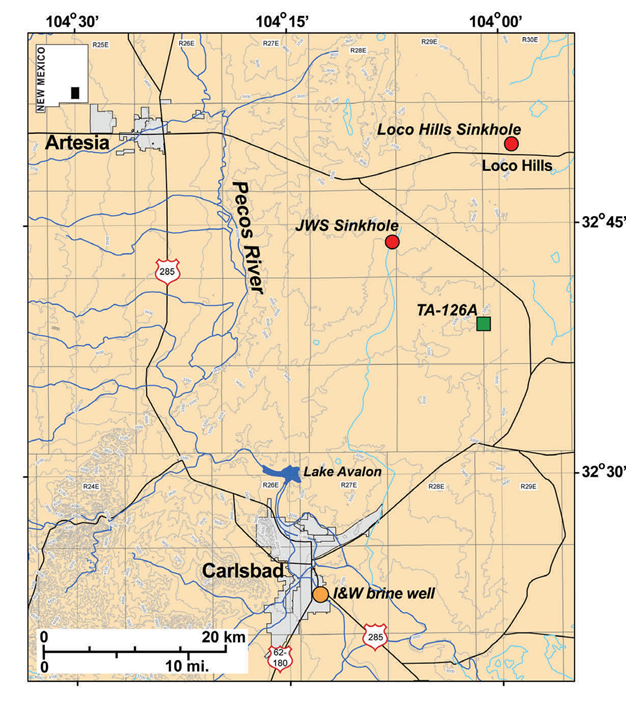
\includegraphics[width=0.8\textwidth]{carlsbad.png}
  \caption{新墨西哥州的卤水井}
  \label{fig:carlsbad}
  \note{注:图片引自\inlinecite{landElectricalResistivitySurvey2011},
  图中JWS Sinkhole和Loco Hills Sinkhole为已经坍塌的卤水井,I\&W Brine Well为未坍塌的卤水井,也是本文的研究区域。}
\end{figure}
\begin{figure}[htb]
    \centering
    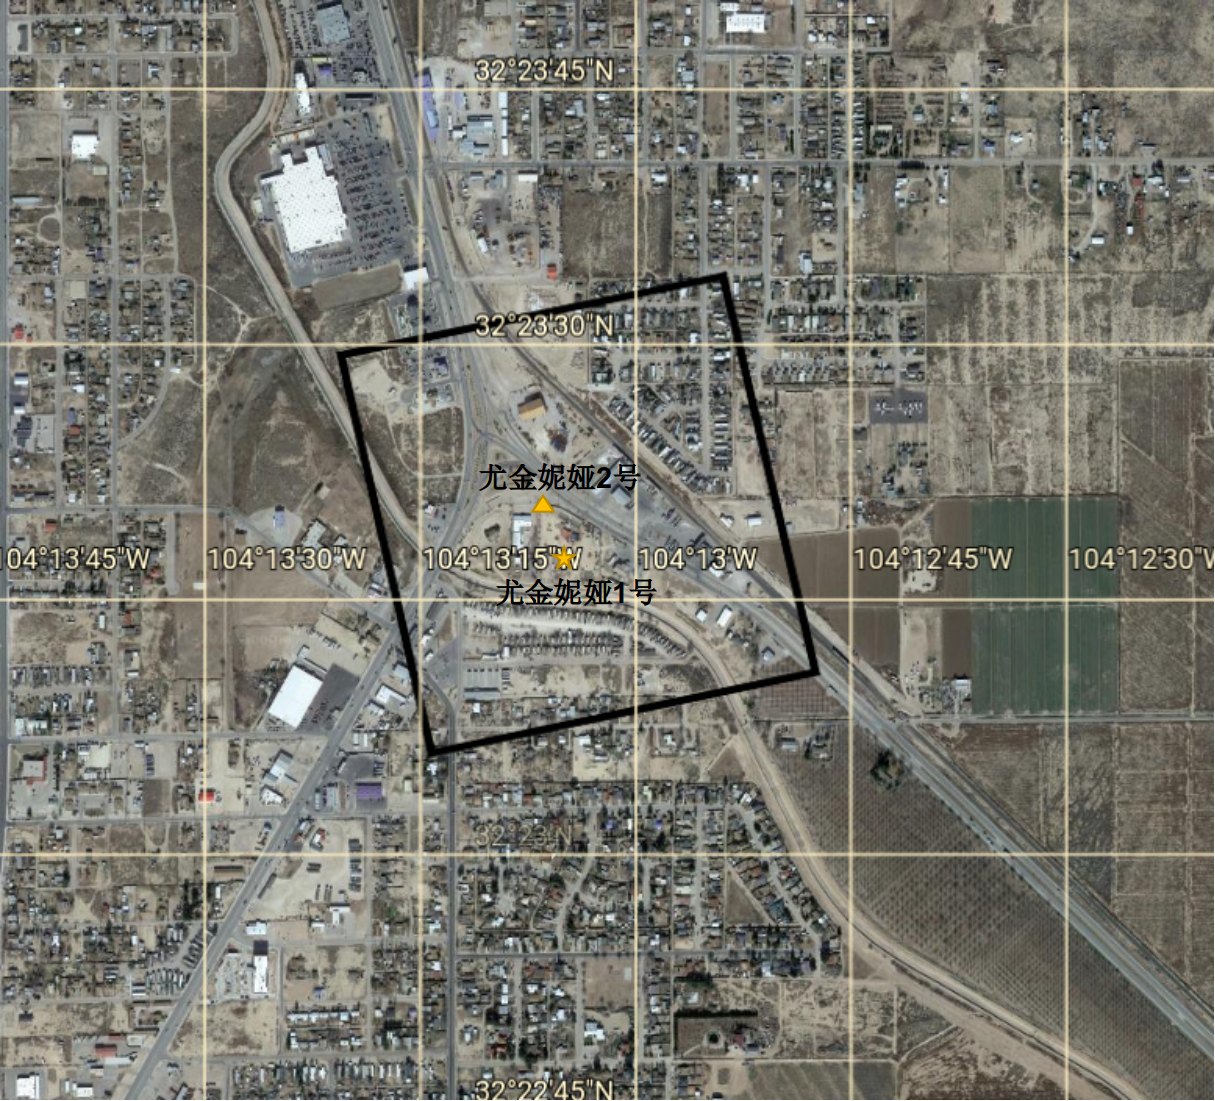
\includegraphics[width=0.8\textwidth]{studyareav2.png}
    \caption{研究区域示意图}
    \note{注:图中三角形所标地点为尤金妮娅2号,正方形所标地点为尤金妮娅1号。}
    \label{fig:studyarea}
\end{figure}
\subsection{地质背景}
研究区域在德州西方,新墨西哥州的东南方的配科斯地区。
配科斯地区为喀斯特地形,其基岩的主要成分为石膏,是典型的石灰岩地区。
该地区石膏基岩上分布有岩溶裂隙和坑洞。
部分坑洞是自然形成的,一般由地下水上涌溶蚀基岩形成,也有部分和盐层的溶浸开采有关。
此卤水井位于特拉华盆地,该盆地的最上部分由约1700m的红层和蒸发岩组成。
该部分包含salado地层,大概在地下140-180m之间,含有丰富的岩盐。
该卤水井的目的就是开采该地层的岩盐。

\subsection{开采背景}
向地下注入新鲜的淡水,等待岩盐充分溶解之后将饱和溶液泵出并提纯,这是此类卤水井的开采原理。
该处卤水井一共有两口井,分别称为尤金妮娅1号和尤金妮娅2号。如图\ref{fig:studyarea}所示。

尤金妮娅1号首先被钻成,并作为单井使用。
然而,由于产量不高的原因,又钻了位于尤金妮娅1号西北方向100米左右的尤金妮娅2号。
之后两个水井被打通,尤金妮娅2号作为淡水注入井,而溶有岩盐的水从尤金妮娅1号泵出。
从2000年开始,尤金妮娅2号被关停,尤金妮娅1号再次作为单井使用。

\section{数据源}

本研究使用的数据为ALOS PALSAR的数据。
ALOS是日本与2006年发射的卫星,PALSAR为该卫星上搭载的L波段的合成孔径雷达。
数据的基本参数见表\ref{tab:palsar}。
% \begin{table}[htb]
%     \centering\small
%     \caption{数据基本参数}
%     \label{tab:palsar}
%     \begin{tabular}{@{}cc@{}}
%     \toprule
%     参数           & 值                                \\ 
%     \midrule
%     雷达           & ALOS PALSAR                      \\
%     中心频率         & 1270 MHz(L波段)                    \\
%     range方向采样数   & 94                               \\
%     azimuth方向采样数 & 252                              \\
%     heading      & $-10.13^{\circ}$至$-10.18^{\circ}$ \\
%     入射角          & $38.73^{\circ}$左右  \\
%     \bottomrule
%     \end{tabular}
% \end{table}
监测时间从2006年12月到2011年2月共计15幅影像,详情参见表\ref{tab:timeseries}。
% \begin{table}[htb]
%     \centering\small
%     \caption{数据时间序列}
%     \label{tab:timeseries}
%     \begin{tabular}{@{}cccc@{}}
%     \toprule
%     序号 & 成像时间 & 序号 & 成像时间\\ 
%     \midrule
%     1 & 2006.12.20 & 9 & 2010.05.15 \\
%     2 & 2007.06.22 & 10 & 2010.06.30 \\
%     3 & 2007.12.23 & 11 & 2010.08.15 \\
%     4 & 2008.05.09 & 12 & 2010.09.30 \\
%     5 & 2008.06.24 & 13 & 2010.11.15 \\
%     6 & 2008.12.25 & 14 & 2010.12.31 \\
%     7 & 2009.12.28 & 15 & 2011.02.15 \\
%     8 & 2010.05.30 & & \\
%     \bottomrule
%     \end{tabular}
% \end{table}
\begin{table}
    \centering\small
    \begin{minipage}{0.8\textwidth}
        \centering\small
    \caption{数据基本参数}
    \label{tab:palsar}
    \begin{tabular}{@{}cc@{}}
    \toprule
    参数           & 值 \\ 
    \midrule
    雷达           & ALOS PALSAR  \\
    中心频率         & 1270 MHz(L波段) \\
    range方向采样数   & 94  \\
    azimuth方向采样数 & 252  \\
    range方向像素步长 & 4.684257m \\
    azimuth方向像素步长 & 3.151791m \\
    heading      & $-10.1971846^{\circ}$至$-10.1293200^{\circ}$ \\
    入射角          & $38.7264^{\circ}$至$38.7419^{\circ}$  \\
    \bottomrule
    \end{tabular}
    \end{minipage}
    \begin{minipage}{0.8\textwidth}
        \centering\small
        \caption{数据时间序列}
        \label{tab:timeseries}
        \begin{tabular}{@{}cccc@{}}
        \toprule
        序号 & 成像时间 & 序号 & 成像时间\\ 
        \midrule
        1 & 2006.12.20 & 9 & 2010.05.15 \\
        2 & 2007.06.22 & 10 & 2010.06.30 \\
        3 & 2007.12.23 & 11 & 2010.08.15 \\
        4 & 2008.05.09 & 12 & 2010.09.30 \\
        5 & 2008.06.24 & 13 & 2010.11.15 \\
        6 & 2008.12.25 & 14 & 2010.12.31 \\
        7 & 2009.12.28 & 15 & 2011.02.15 \\
        8 & 2010.05.30 & & \\
        \bottomrule
        \end{tabular}   
    \end{minipage}
\end{table}

\section{数据处理}

\subsection{预处理}
本研究首先使用gamma软件进行干涉对的选择,选取2009年12月28日的影像为超级主影像,
设置时间基线阈值为1250天,空间基线阈值为1450米,一共构建67对干涉对。
其中最大时间基线为1242天,最小时间基线为46天;
最大空间基线为1499.7米,最小空间基线为6米。
结果如图\ref{fig:bprep}所示。
\begin{figure}[htb]
    \centering
    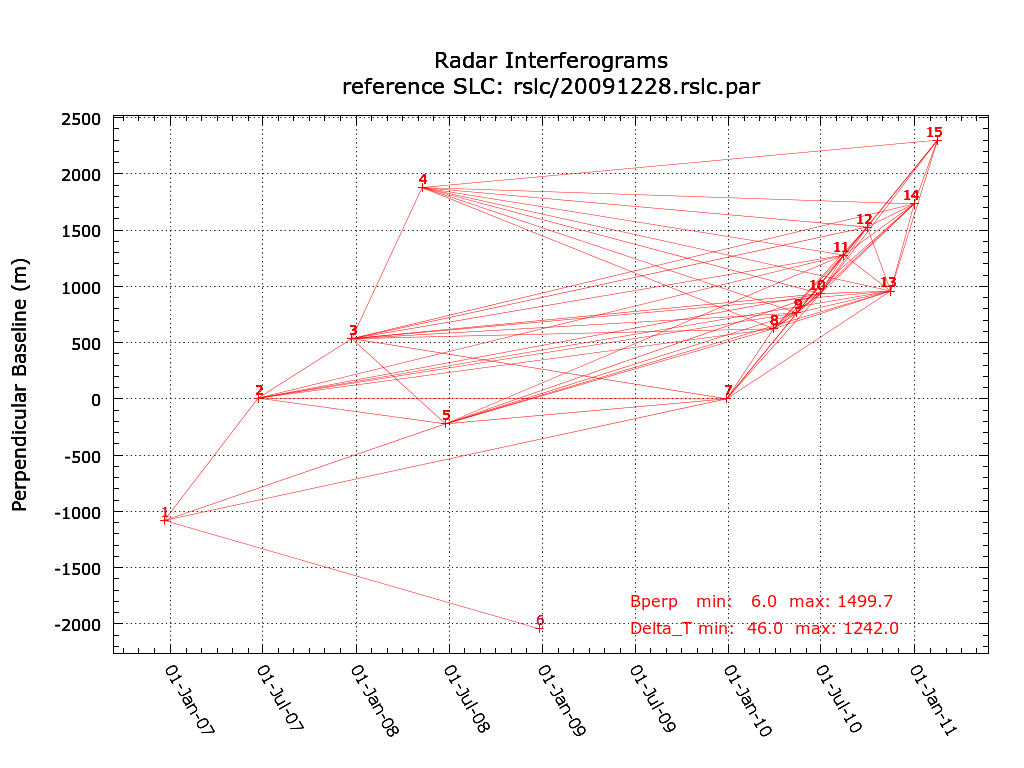
\includegraphics[width=0.8\textwidth]{bperp.png}
    \caption{时空基线连接图}
    \label{fig:bprep}
\end{figure}

干涉对选择好以后,将所有的影像和超级主影像配准,
所谓配准,就是把其他影像的数据归算到超级主影像的坐标中。
之后将配准的影像做干涉处理,并利用DEM去除地形效应。
这里使用的DEM数据为1弧秒的SRTM DEM数据。

\subsection{SBAS处理}
之后使用StamPS软件进行SBAS技术数据处理。
SBAS的处理流程如图\ref{fig:sbasflow}所示。
\begin{figure}[htb]
    \centering
    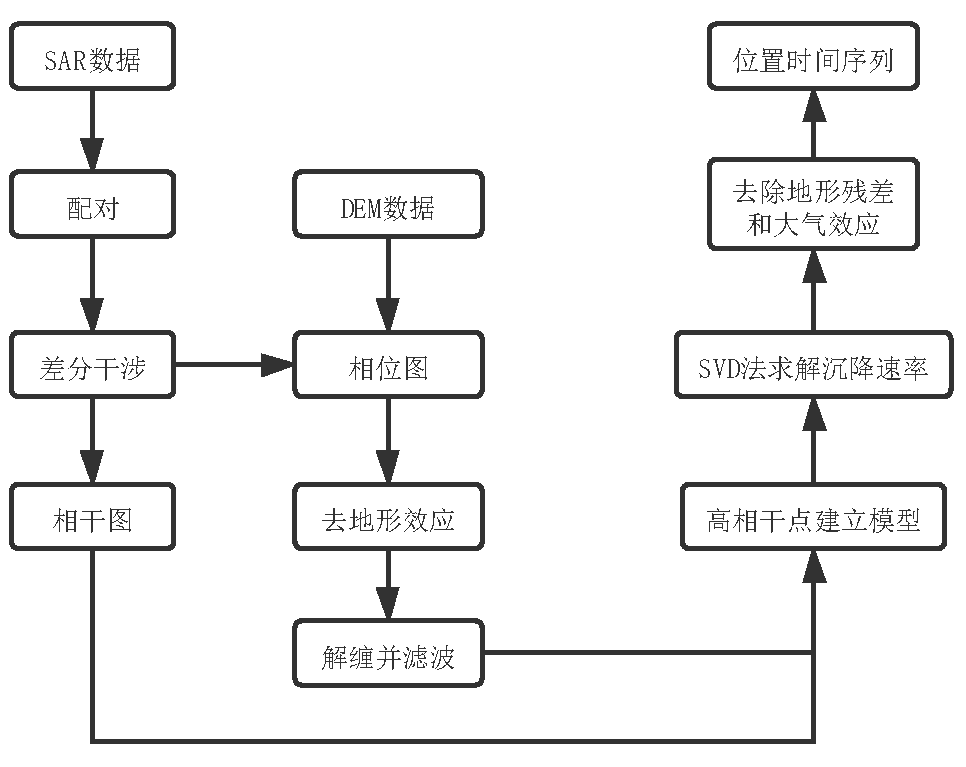
\includegraphics[width=0.8\textwidth]{sbasflow.pdf}
    \caption{SBAS处理流程图}
    \label{fig:sbasflow}
\end{figure}

处理所得平均速度如图\ref{fig:sbasv},相对的形变如图\ref{fig:sbasu}所示。
\begin{figure}[htb]
    \centering
    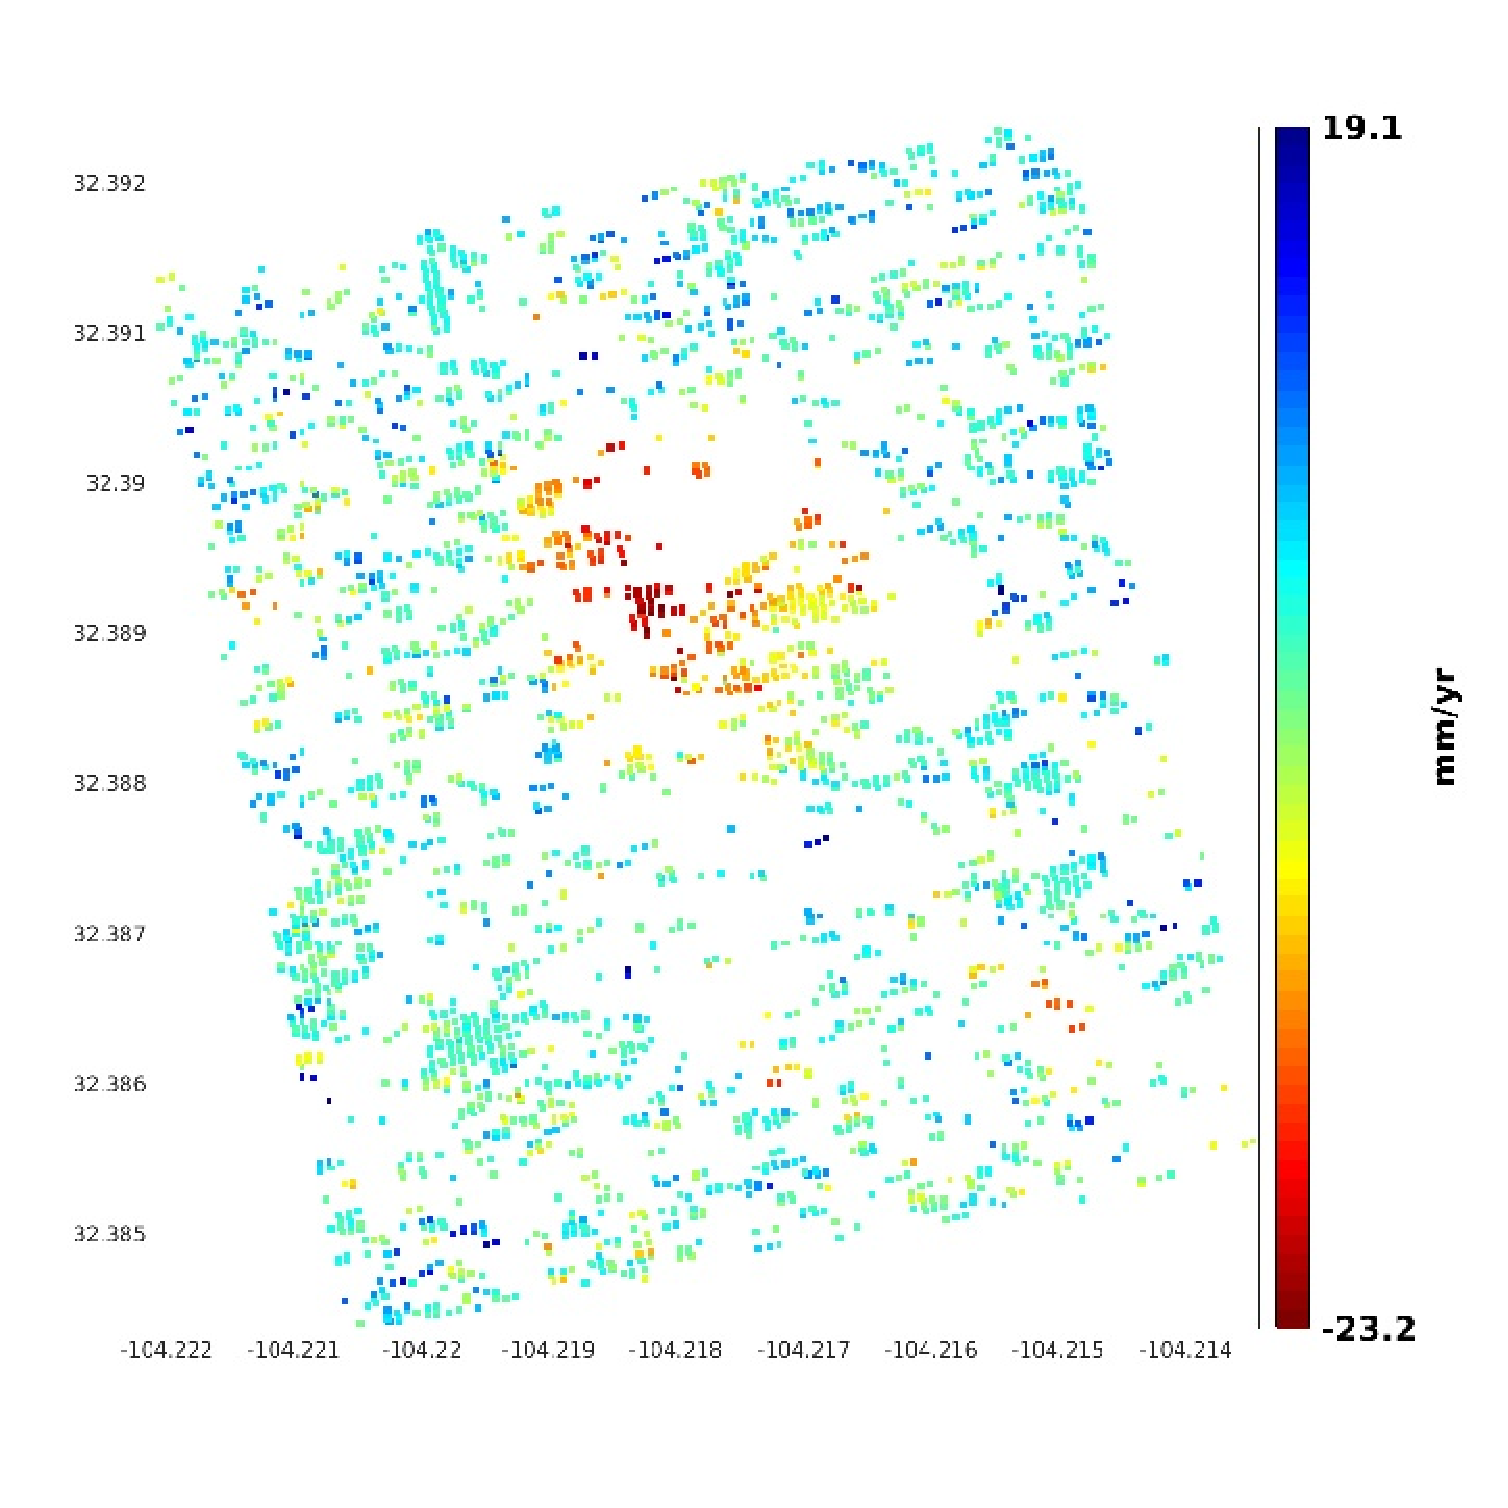
\includegraphics[width=1.0\textwidth]{sbasv.eps}
    \caption{研究区域平均沉降速率图}
    \label{fig:sbasv}
\end{figure}
\begin{figure}[htb]
    \centering
    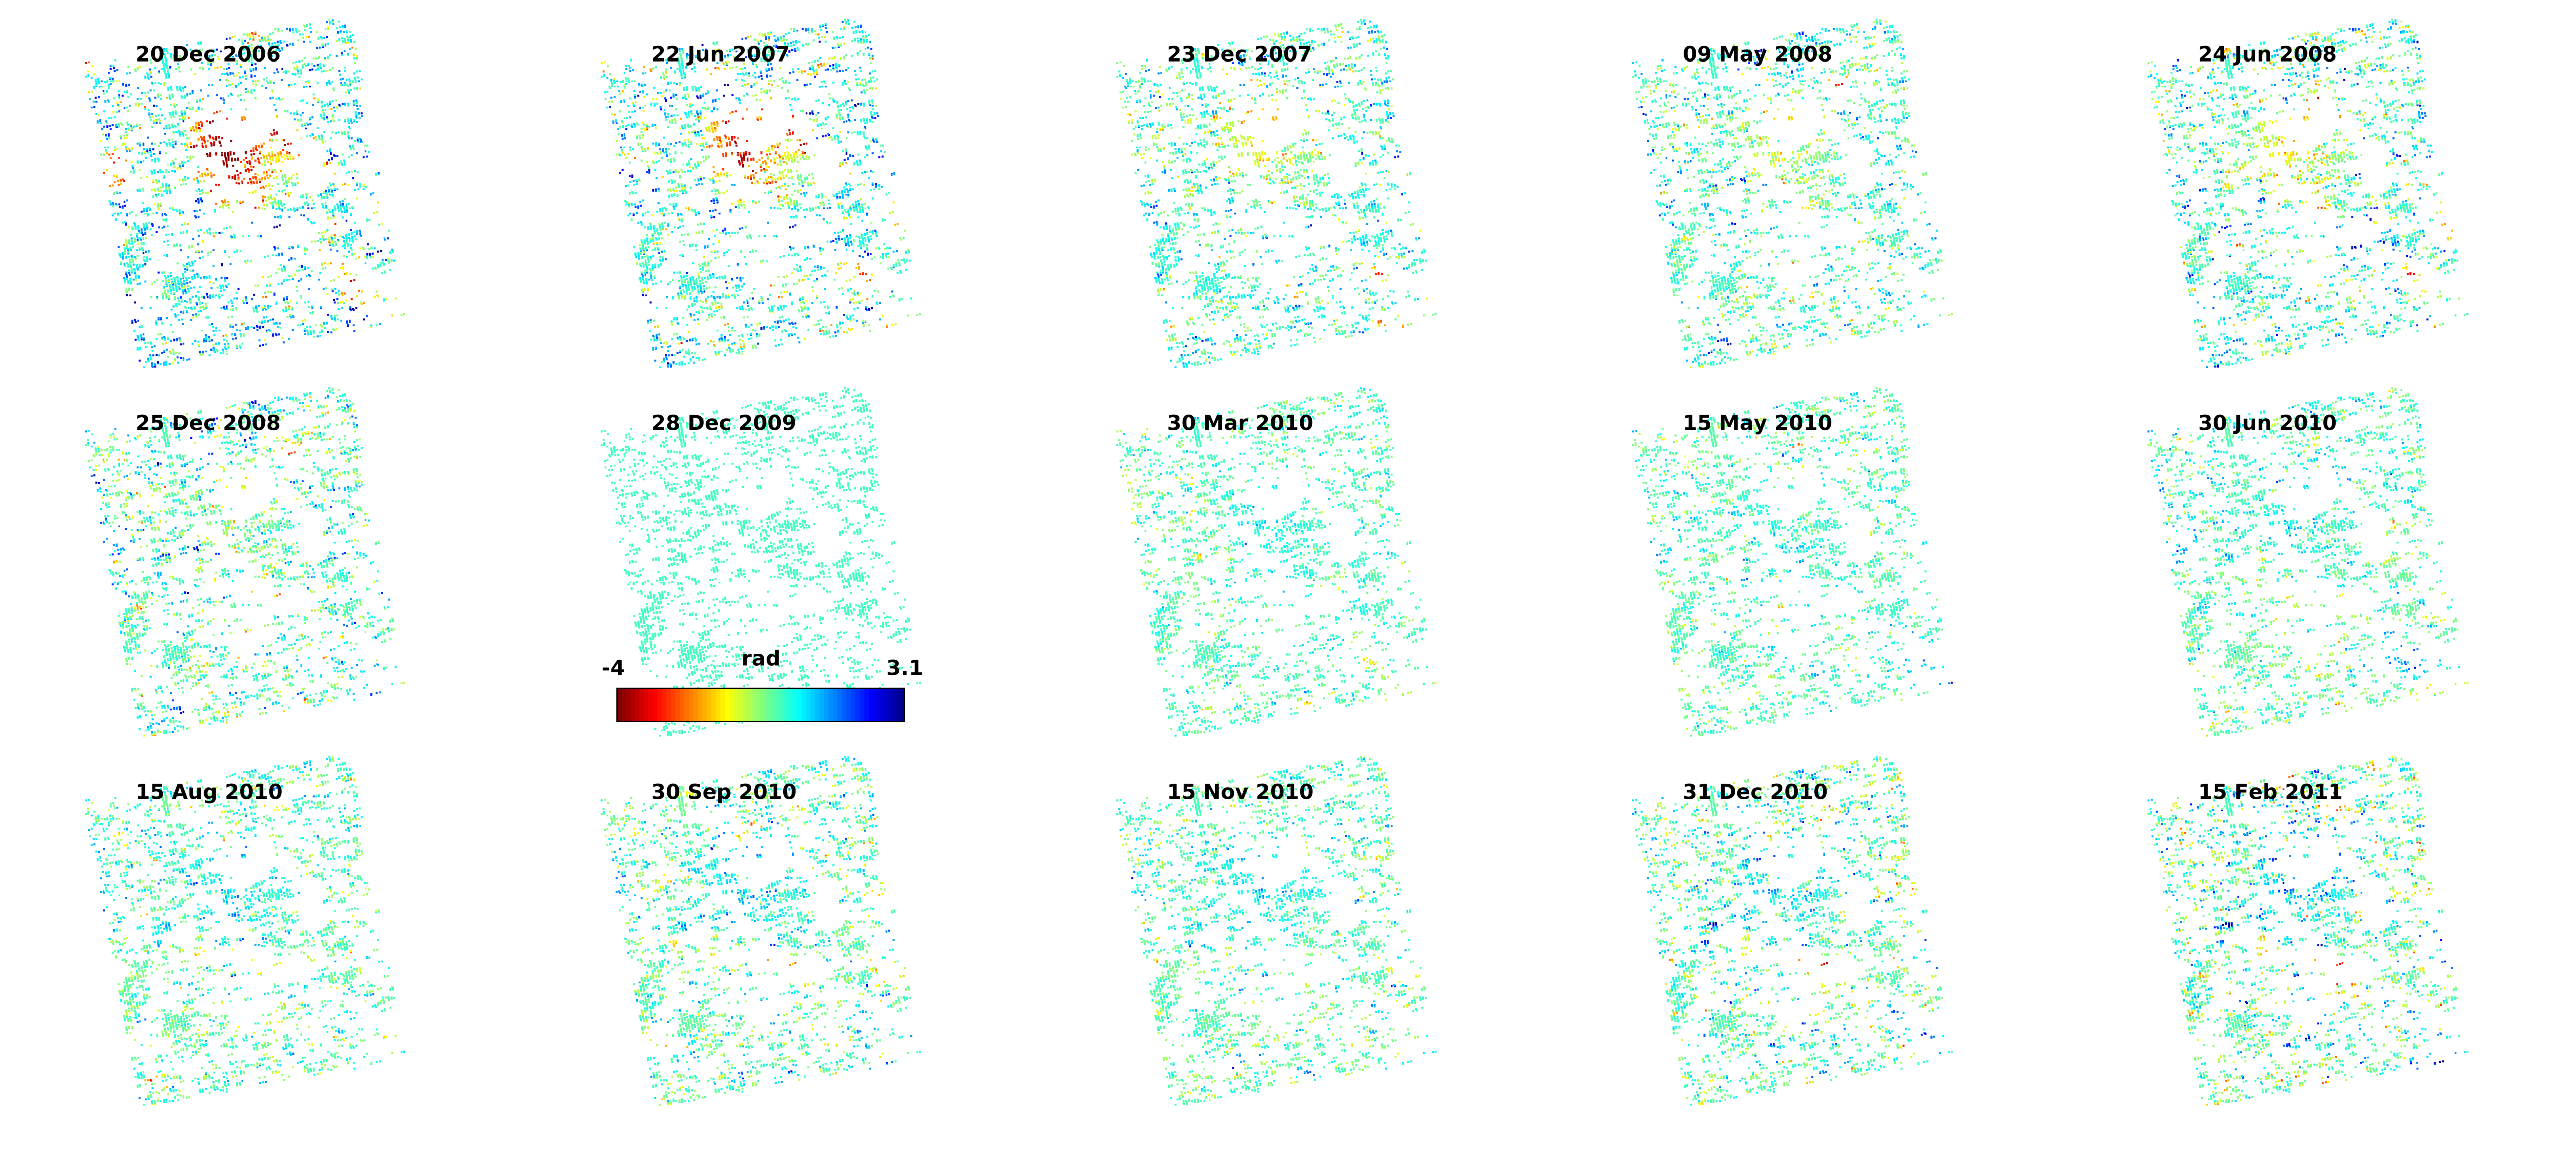
\includegraphics[width=1.0\textwidth]{sbasu.pdf}
    \caption{研究区域相对于主影像形变图}
    \label{fig:sbasu}
\end{figure}

\section{形变结果的初步分析}
从图\ref{fig:sbasv}和图\ref{fig:sbasu}中可以明显地看出中部区域有明显的沉降。
变形最明显的区域的形变可以达到平均23.2mm/year的速度,
累计最大形变可达81mm。
从形变的结果来看,此变形比较类似于点源引起的变形,该点源的位置大概在尤金妮娅1号所在的位置,
初步估计此处的沉降是尤金妮娅1号的开采导致的地下空洞引发的次生灾害。
同时,右下角部分有一定的形变,但由于在该部位所选取的PS点较少的缘故,该区域的形变很难建模。
下一步的研究将使用点源对形变做一个物理模型并分析模型和实际空洞的差别。